% This is a general template file for the LaTeX package SVJour3
% for Springer journals. Original by Springer Heidelberg, 2010/09/16
%
% Use it as the basis for your article. Delete % signs as needed.
%
% This template includes a few options for different layouts and
% content for various journals. Please consult a previous issue of
% your journal as needed.
%
\RequirePackage{fix-cm}
%
%\documentclass{svjour3}                     % onecolumn (standard format)
%\documentclass[smallcondensed]{svjour3}     % onecolumn (ditto)
%\documentclass[smallextended]{svjour3}       % onecolumn (second format)
\documentclass[twocolumn]{svjour3}       % onecolumn (second format)
%
\smartqed  % flush right qed marks, e.g. at end of proof
%
\usepackage{graphicx}
%
% insert here the call for the packages your document requires
%\usepackage{mathptmx}      % use Times fonts if available on your TeX system
%\usepackage{latexsym}
\usepackage{natbib}
\usepackage{multirow}
\usepackage{gensymb}
\usepackage{hyphenat}
\usepackage[mathlines]{lineno}

\journalname{Climate Dynamics}
\date{}
%

\def\makeheadbox{{%
		\hbox to0pt{\vbox{\baselineskip=10dd\hrule\hbox
				to\hsize{\vrule\kern3pt\vbox{\kern3pt
						\hbox{\bfseries\ Climate Dynamics -- Supplementary material}
						\kern3pt}\hfil\kern3pt\vrule}\hrule}%
			\hss}}}
%

\newcommand{\beginsupplement}{%
	\renewcommand{\thetable}{S\arabic{table}}%
	\renewcommand{\thefigure}{S\arabic{figure}}%
	\renewcommand{\thesection}{S\arabic{section}}%
}



\begin{document}
	
	\title{Supplementary material to: Impact of global atmospheric reanalyses on statistical precipitation downscaling
		%\thanks{}
	}
	% Grants or other notes about the article that should go on the front
	% page should be placed within the \thanks{} command in the title
	% (and the %-sign in front of \thanks{} should be deleted)
	%
	% General acknowledgments should be placed at the end of the article.
	
	%\subtitle{Do you have a subtitle?\\ If so, write it here}
	
	%\titlerunning{Short form of title}        % if too long for running head
	
	\author{Pascal Horton         \and
		Stefan Br\"{o}nnimann
	}


	%\affiliation{Oeschger Centre for Climate Change Research, Institute of Geography, University of Bern, Bern, Switzerland}
	
	%\authorrunning{Short form of author list} % if too long for running head
	
	\institute{P. Horton \at
		University of Bern,
		Hallerstrasse 12, 
		3012 Bern, 
		Switzerland \\
		Tel.: +41 31 631 80 21\\
		\email{pascal.horton@giub.unibe.ch}\\
		ORCID: 0000-0003-0466-0359           %  \\
		%             \emph{Present address:} of F. Author  %  if needed
		\and
		S. Br\"{o}nniman \at
		University of Bern,
		Hallerstrasse 12, 
		3012 Bern, 
		Switzerland
	}
	
	\maketitle
	
	\beginsupplement
	

	\section{Selection of the analogue dates for different precipitation thresholds}
	\label{supp:analogue_days}
	
	The selection of the analogue dates were compared between reanalyses for all stations and all AMs for different precipitation thresholds. Figure \ref{fig:similarities_analogue_dates_0} shows the percentage of identical analogue dates selected when using the reanalyses in columns that were also found when using the reanalyses in rows for the different AMs and for the target dates with non null precipitation. Figure \ref{fig:similarities_analogue_dates_095} and Fig. \ref{fig:similarities_analogue_dates_099} show the same information but for days with precipitation above the $95^{th}$ or $99^{th}$ percentiles of non null precipitation. For days with higher precipitation, the percentage of common analogue dates tend to increase, but not to substantial extent. Overall, the patterns remains similar.	
	
	\begin{figure}
		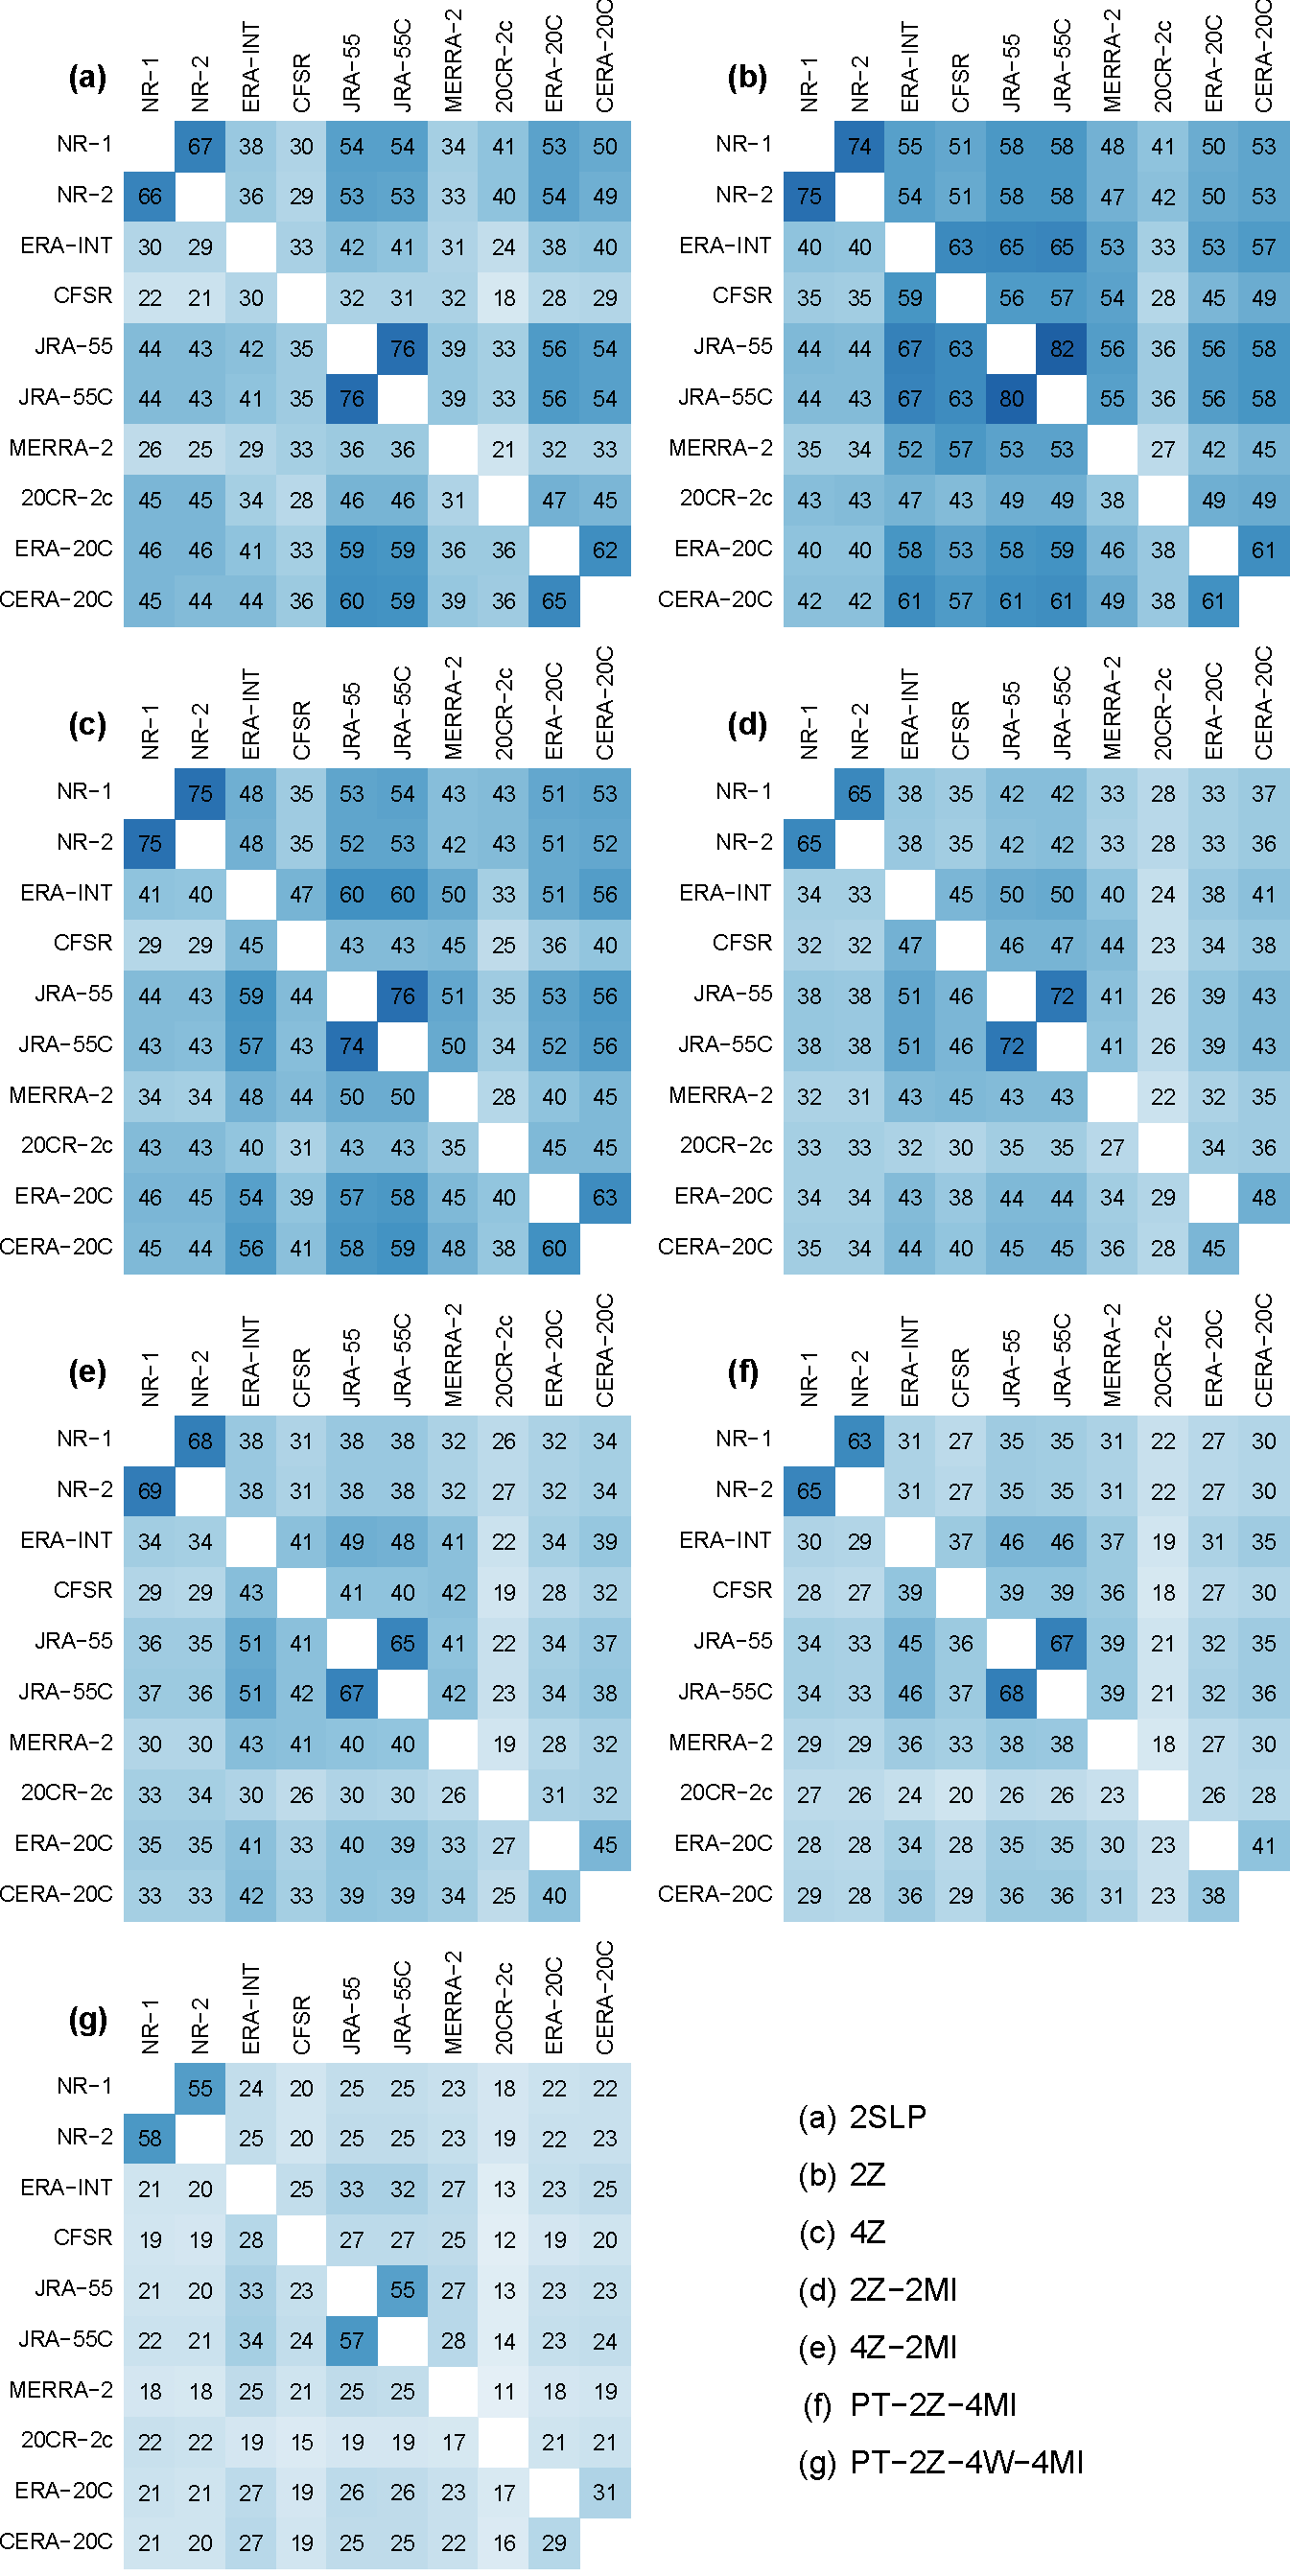
\includegraphics[width=0.48\textwidth]{figure-supp-dates-thres-0.pdf}\\
		\caption{Percentage of identical analogue dates selected when using the reanalysis datasets in columns that are also found when using the datasets in rows for different AMs. The values are averaged for all stations on the VP, but only for target dates with a non null precipitation.}
		\label{fig:similarities_analogue_dates_0}
	\end{figure}
	
	\begin{figure}
		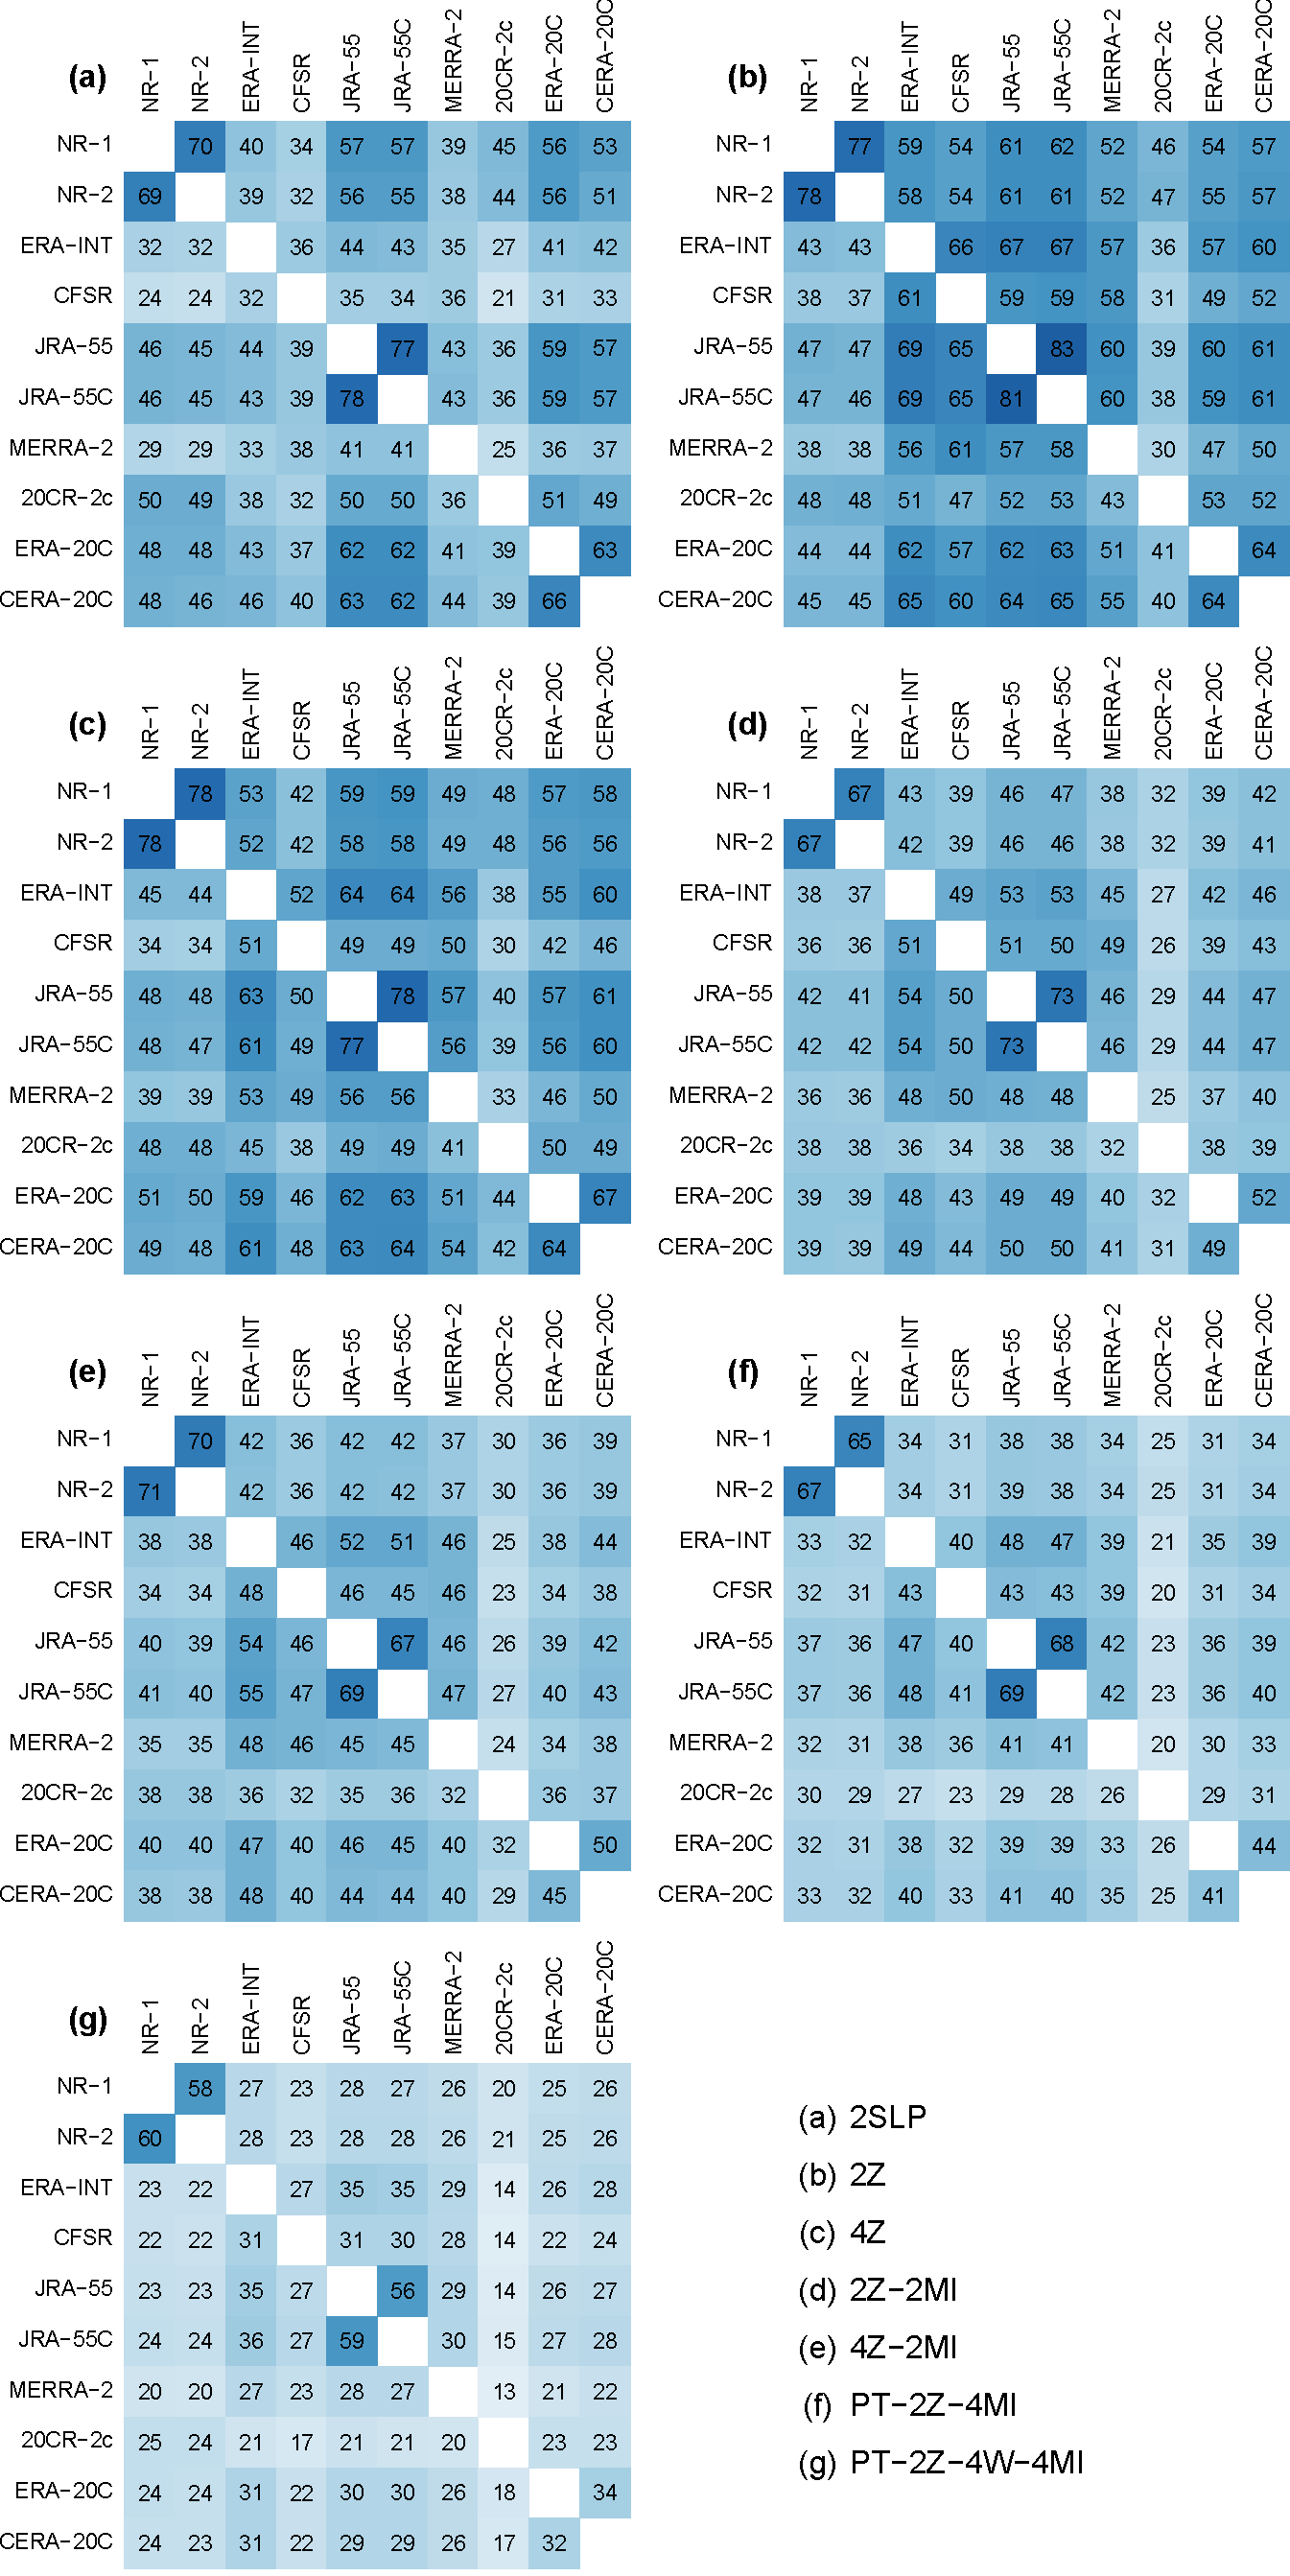
\includegraphics[width=0.48\textwidth]{figure-supp-dates-thres-095.pdf}\\
		\caption{Same as \ref{fig:similarities_analogue_dates_0} but for target dates with precipitation above the $95^{th}$ percentile of non null precipitation.}
		\label{fig:similarities_analogue_dates_095}
	\end{figure}

	\begin{figure}
		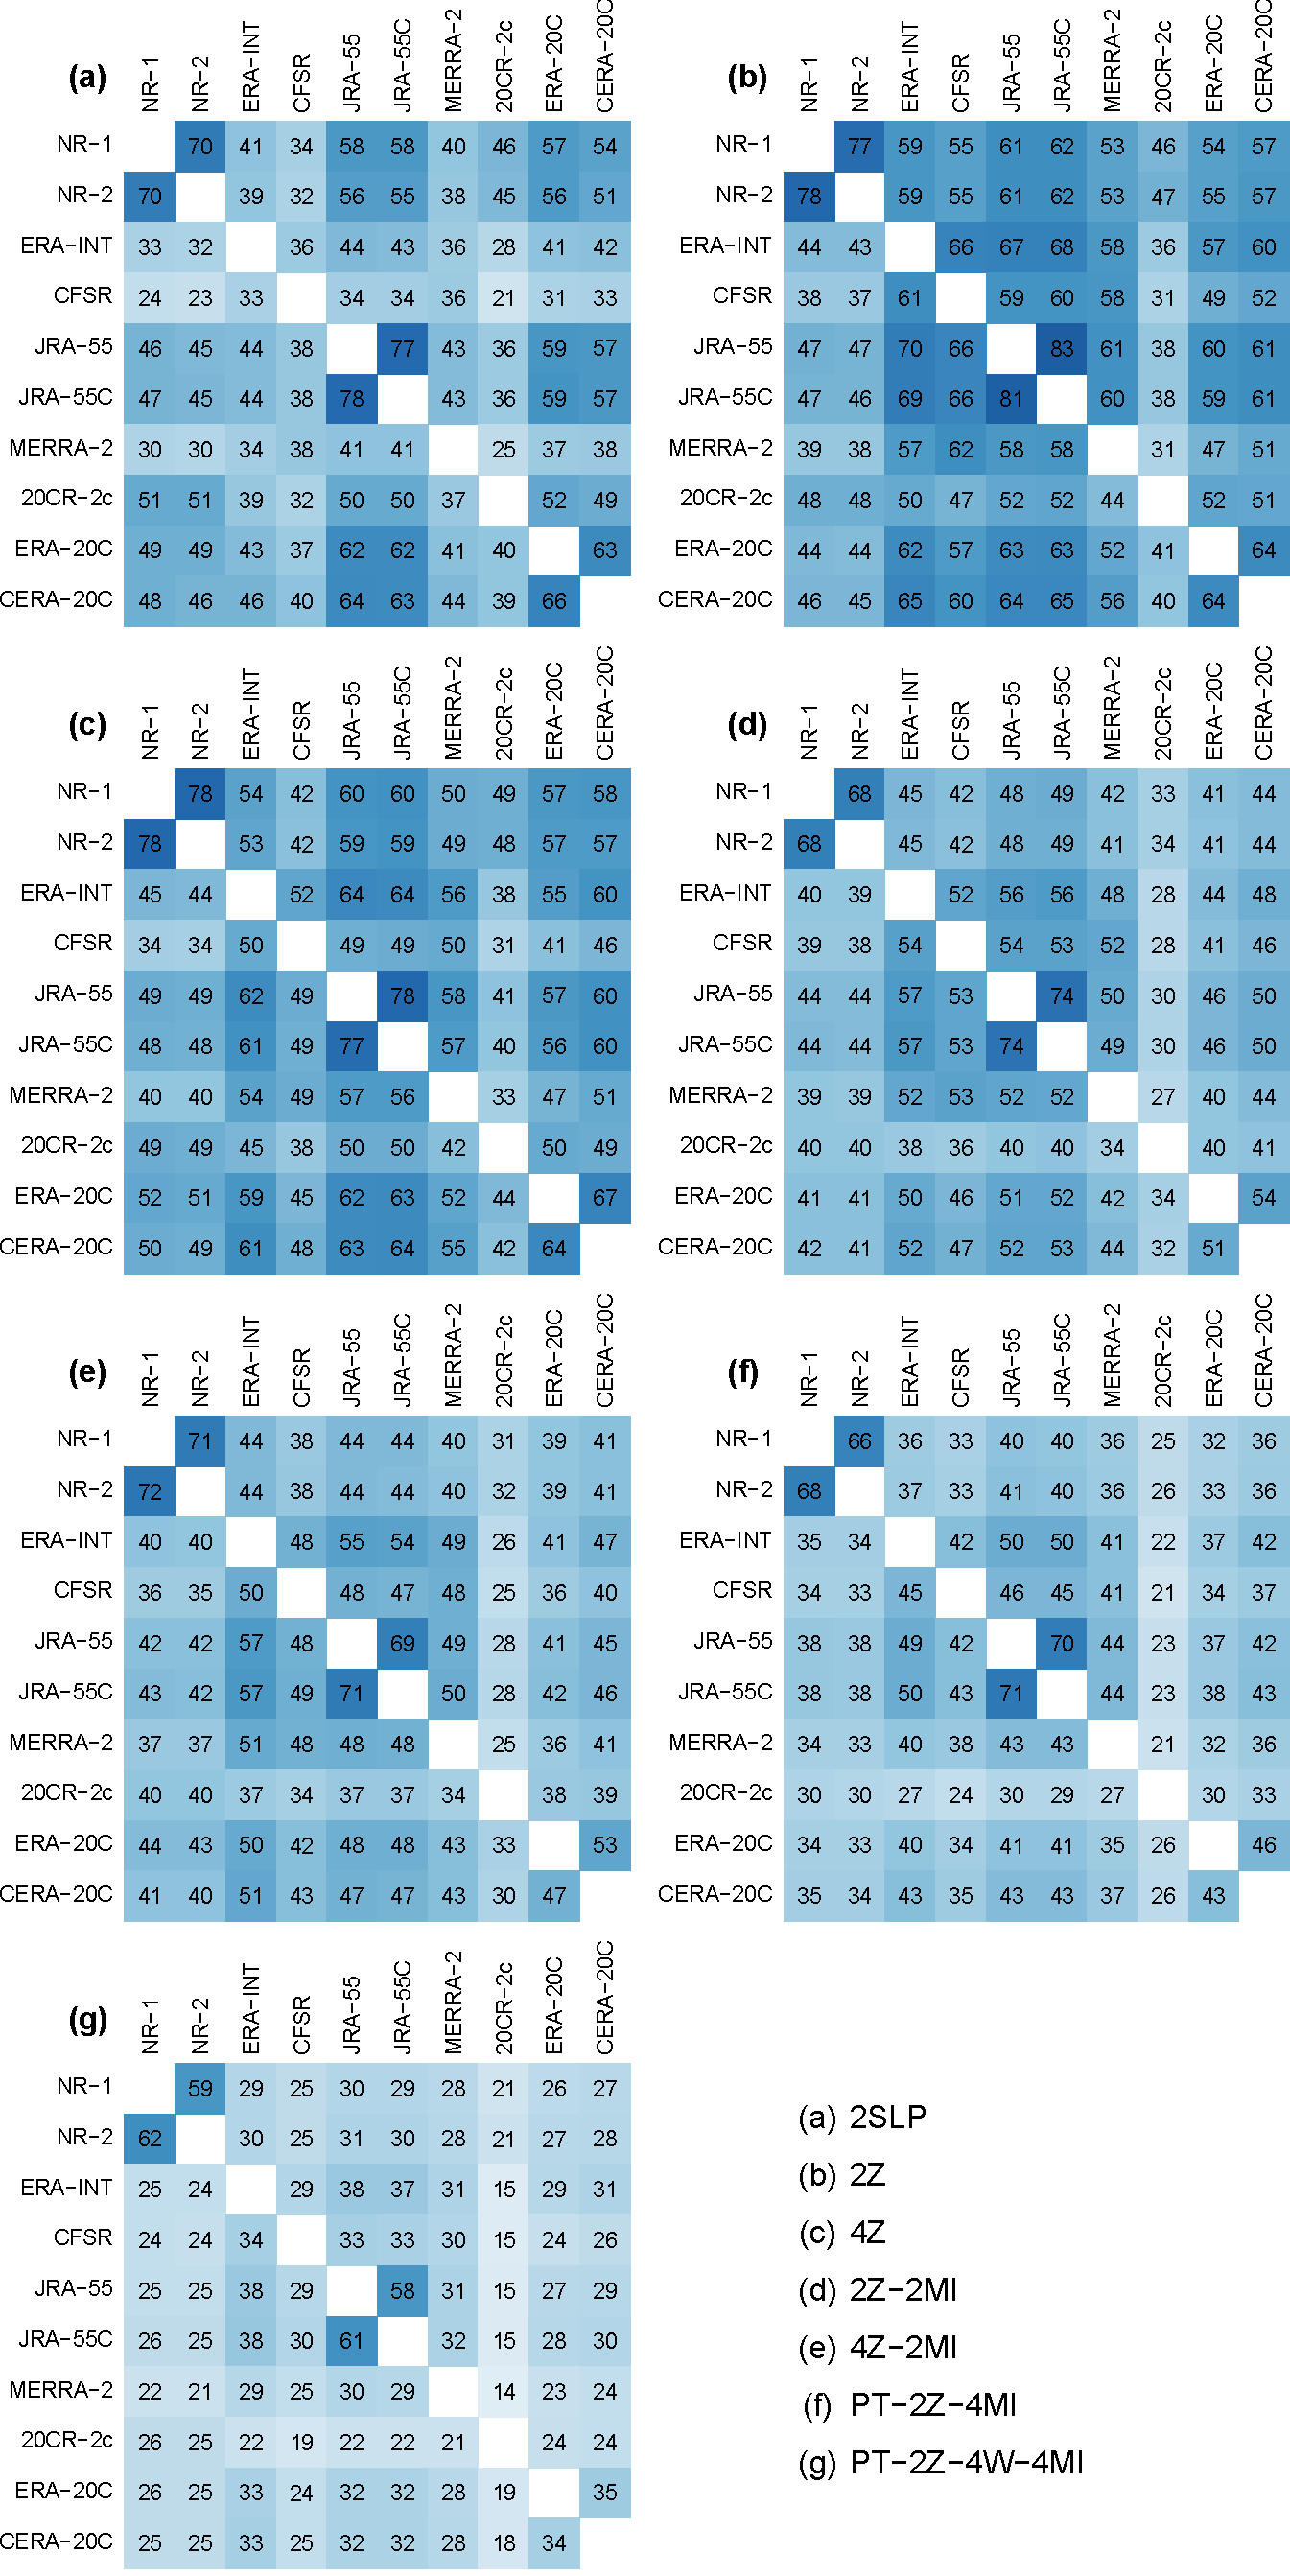
\includegraphics[width=0.48\textwidth]{figure-supp-dates-thres-099.pdf}\\
		\caption{Same as \ref{fig:similarities_analogue_dates_0} but for target dates with precipitation above the $99^{th}$ percentile of non null precipitation.}
		\label{fig:similarities_analogue_dates_099}
	\end{figure}

	
	
\end{document}
